\section{APPENDIX}

\subsection{Determine parameters of air}
On the $I$-$d$ diagram, based on wet bulb and dry bulb temperature, the following procedure is used to determine Relative Humidity $\varphi$ (\%), Enthalpy $I$ (kJ/kg), and Density $d$ (kg/kg) of the air at different points:
\begin{enumerate}
    \item Draw a vertical line through $t_{wet}$, parallel to $t = \text{const}$, intersecting $\varphi = 1$ at point A.
    \item Draw a vertical line through $t_{dry}$, parallel to $t = \text{const}$.
    \item Draw a line through point A, parallel to $I = \text{const}$ (this line shows the enthalpy $I$ values at different states), intersecting the $t_{dry}$ line at point B.
    \item B is the point indicating the state of air determined by $t_{wet}$ and $t_{dry}$ values.
    \item The $\varphi = 0$ line through B shows the Relative Humidity $\varphi$ value of air.
\end{enumerate}

\begin{figure}[H]
    \centering
    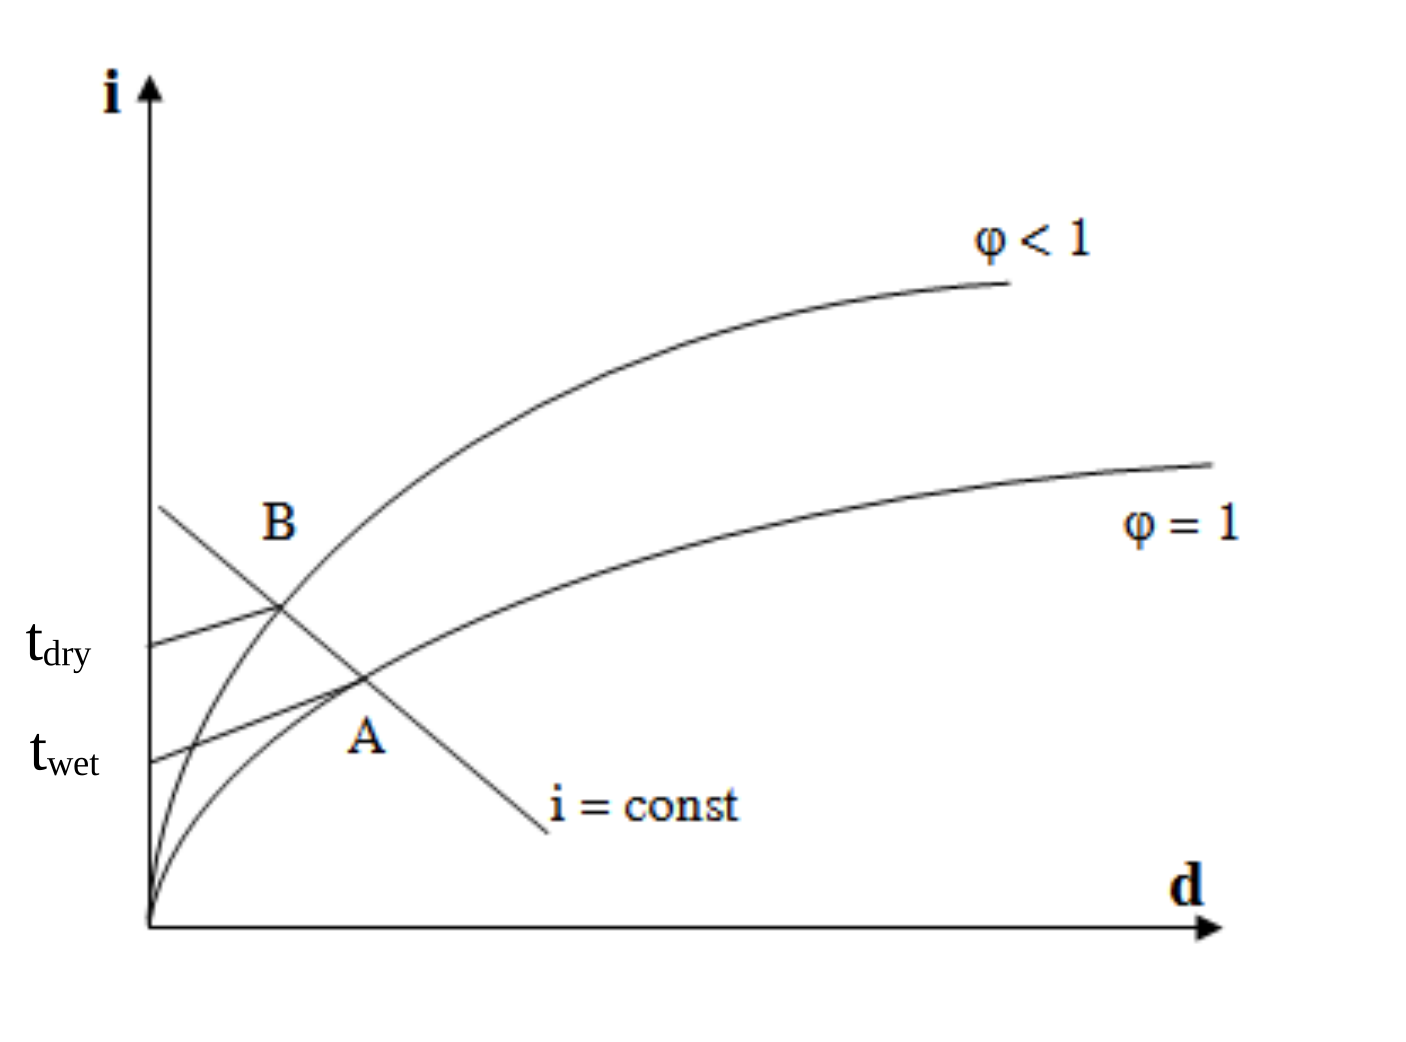
\includegraphics[width=0.65\linewidth]{Images/figure11.png}
    \caption{Way to determine parameters of air, knowing wet bulb and dry bulb temperature.}
    \label{fig:id_appendix}
\end{figure}

\noindent The relative humidity is calculated using the psychrometric formula:
\begin{equation}
    \varphi = \frac{p_m}{p_b} - \frac{A \cdot B}{p_b}(t_{dry} - t_{wet})
\end{equation}
where $p_m$ and $p_b$ are saturation pressures at wet and dry bulb temperatures respectively, and $A = 66 \times 10^{-5}$ for $v < 0.5$ m/s.

\noindent Absolute humidity $d$:
\begin{equation}
    d = \frac{18}{29} \times \frac{\varphi \cdot p_b}{B - \varphi \cdot p_b}
\end{equation}

\noindent Enthalpy:
\begin{equation}
    I = t_{dry} + (2493 + 1.97 \cdot t_{dry}) \cdot d \quad \text{(kJ/kg)}
\end{equation}

\subsection{Determine the air flowrate passing through the Aerodynamic tube}
Mass flowrate $G_{kk}$ (kg/s) of air in aerodynamic tube can be determined using the following formula:
\begin{equation}
    G_{kk} = v \cdot F \cdot \rho \quad \text{(kg/s)}
\end{equation}
Where:
\begin{itemize}
    \item $v$: velocity of the air measured at the outlet of aerodynamic tube, m/s.
    \item $F = 0.0144$ m$^2$: the outlet area of aerodynamic tube.
    \item $\rho$: specific mass of air (from Table \ref{tab:airdensity}), kg/m$^3$.
\end{itemize}

\begin{table}[H]
\centering
\caption{Specific mass of air $\rho$ (kg/m$^3$) as a function of temperature ($^\circ$C)}
\label{tab:airdensity}
\begin{tabular}{|c|c|c|c|c|c|c|c|c|c|c|}
\hline
\textbf{t ($^\circ$C)} & 30 & 31 & 32 & 33 & 34 & 35 & 36 & 37 & 38 & 39 \\ \hline
$\rho$ (kg/m$^3$) & 1.165 & 1.161 & 1.157 & 1.154 & 1.150 & 1.146 & 1.142 & 1.139 & 1.135 & 1.131 \\ \hline
\textbf{t ($^\circ$C)} & 40 & 41 & 42 & 43 & 44 & 45 & 46 & 47 & 48 & 49 \\ \hline
$\rho$ (kg/m$^3$) & 1.128 & 1.124 & 1.121 & 1.117 & 1.114 & 1.110 & 1.107 & 1.103 & 1.100 & 1.096 \\ \hline
\textbf{t ($^\circ$C)} & 50 & 51 & 52 & 53 & 54 & 55 & 56 & 57 & 58 & 59 \\ \hline
$\rho$ (kg/m$^3$) & 1.093 & 1.089 & 1.086 & 1.083 & 1.079 & 1.076 & 1.073 & 1.070 & 1.066 & 1.063 \\ \hline
\textbf{t ($^\circ$C)} & 60 & 61 & 62 & 63 & 64 & 65 & 66 & 67 & 68 & 69 \\ \hline
$\rho$ (kg/m$^3$) & 1.060 & 1.057 & 1.054 & 1.051 & 1.047 & 1.044 & 1.041 & 1.039 & 1.035 & 1.032 \\ \hline
\end{tabular}
\end{table}

\subsection{Calculation for cooler}
\textbf{a. Cooling capacity of cooler $Q_0$:}
\begin{equation}
    Q_0 = G_{kk} (I_1 - I_2) \quad \text{(kW)}
\end{equation}
Where $I_1, I_2$: enthalpy of air before and after the cooler (kJ/kg).

\vspace{0.3cm}
\textbf{b. Theoretical volume of water condensed from the cooler $G_{water}$:}
\begin{equation}
    G_{water} = 3600 \cdot G_{kk} \cdot (d_1 - d_2) \quad \text{(kg/h)}
\end{equation}
Where $d_1, d_2$: density of the air before and after the cooler (kg/kg).

\vspace{0.3cm}
\textbf{c. Practical volume of water condensed from the cooler $G'_{water}$:}
\begin{equation}
    G'_{water} = \frac{0.06 \cdot V_1}{t_1} \quad \text{(kg/h)}
\end{equation}
Where $V_1$: volume of water condensed from the cooler (ml); $t_1$: time taken to get water sample (min).

\vspace{0.3cm}
\noindent \textbf{Note:} As we do the experiment twice to get more accurate result, we calculate the average flowrate from 2 experiments before substituting into the equation above.

\subsection{Calculation for Air dryer}
\textbf{a. Heat load $Q$ of Air Dryer:}
\begin{equation}
    Q = G'_{kk} (I_3 - I_2) \quad \text{(kW)}
\end{equation}
Where $I_2, I_3$: enthalpy of air before and after the air dryer (kJ/kg); $G'_{kk}$: mass flowrate of air before the dryer (kg/s).

\vspace{0.3cm}
\textbf{b. The amount of heat generated by the power supply through the resistor:}
\begin{itemize}
    \item $Q' = 1$ kW (one resistor)
    \item $Q' = 2$ kW (two resistors)
\end{itemize}
